\section{Methodology}\label{sec:methodology}
\begin{figure}[t]
\centering
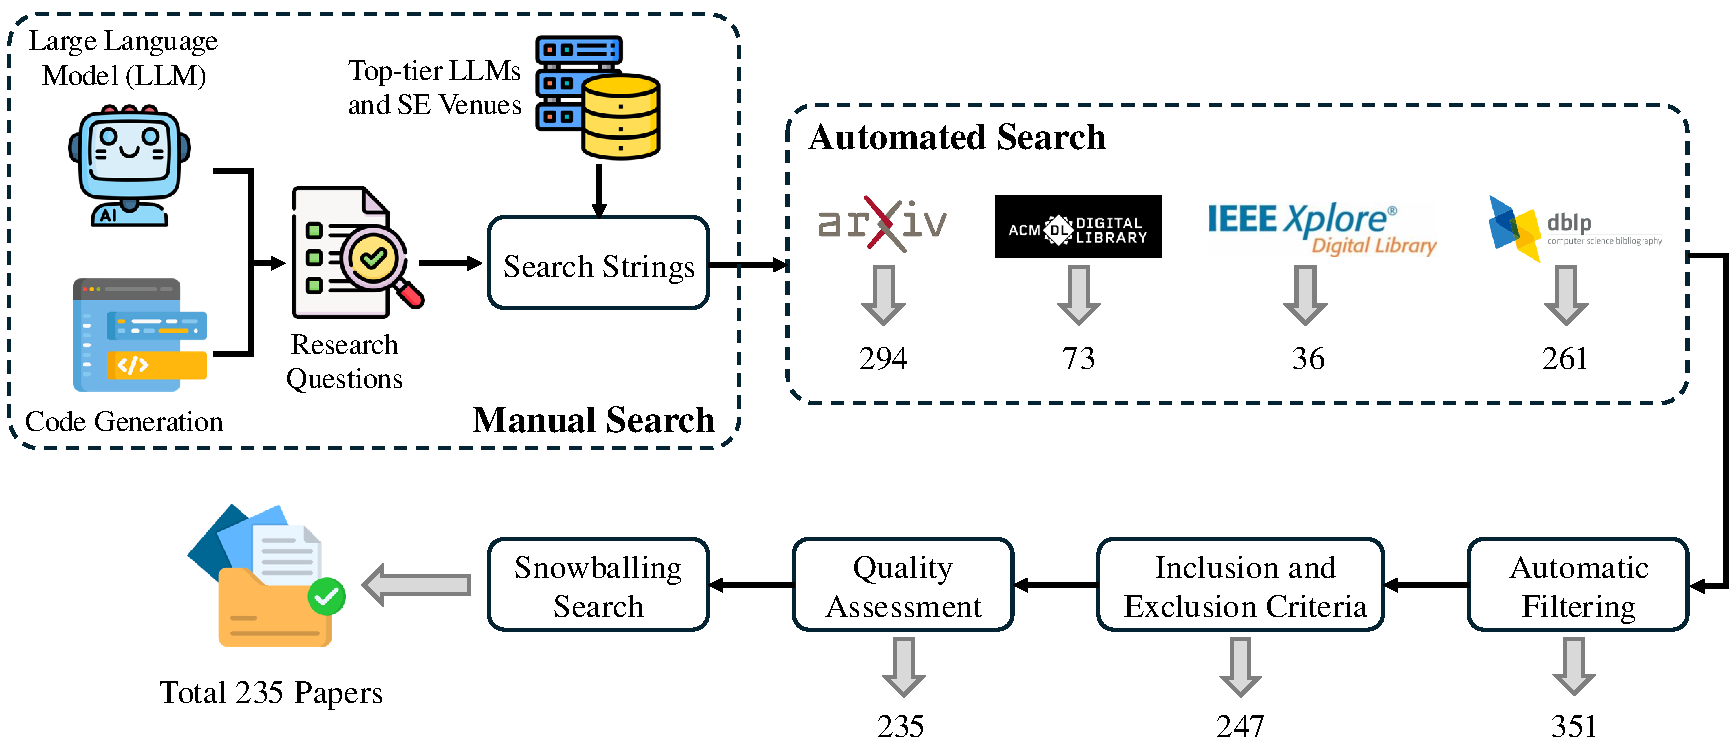
\includegraphics[width=1\linewidth]{images/paper_search_collect_process.pdf}
\caption{\done{Overview of the paper search and collection process.}}
\label{fig:review_process}
\end{figure}

% In this section, we illustrate the details of systematic methodologies for conducting the literature reviews. 
% We follows the systematic literature reviews methodology proposed by \cite{kitchenham2009systematic}, which has been widely used in many software engineering systematic literature review \cite{hou2024large,li2017static,liu2022deep,ramirez2018systematic,wang2022machine}.
% The overall process is depicted in Figure \ref{fig:review_process} and the detailed steps in our methodology are documented below.
In this section, we detail the systematic methodologies employed in conducting literature reviews. We follow the systematic literature review methodology outlined by \cite{kitchenham2009systematic}, which has been widely adopted in numerous software engineering literature reviews \cite{hou2024large,li2017static,liu2022deep,ramirez2018systematic,wang2022machine}. 
The overall process is illustrated in Figure \ref{fig:review_process}, and the detailed steps in our methodology are documented below.

\subsection{Research Questions}
% To provide a comprehensive and up-to-date literature review, and cutting-edge progress dedicated to LLM for code generation, this systematic literature review aims to answer the following research questions (RQs):
To deliver a comprehensive and up-to-date literature review on the latest advancements in large language models (LLMs) for code generation, this systematic literature review addresses the following research questions (RQs):

% \textbf{RQ1: How can we categorize and evaluate the latest advances in LLMs for code generation?}
% The recent surge in the development of LLMs has led to a significant number of these models being repurposed for code generation task. 
% Basically, the adaptation of LLM to code generation follow the evolution of LLMs. However, the evolution of LLMs involves a wide spectrum of research directions and advancements. 
% In particular, it may difficult and laborious for SE researcher to follow comprehensive research evolution of LLM and its adaption to code generation.
% Therefore, RQ1 aims to propose a taxonomy to serves as a comprehensive reference for researchers seeking to quickly familiarize themselves with the state-of-the-art in this dynamic field and pinpoint the specific research problems and directions they are interested in.
\textbf{RQ1: How can we categorize and evaluate the latest advances in LLMs for code generation?}
The recent proliferation of LLMs has resulted in many of these models being adapted for code generation task. 
While the adaptation of LLMs for code generation essentially follows the evolution of LLMs, this evolution encompasses a broad spectrum of research directions and advancements. 
For software engineering (SE) researchers, it can be challenging and time-consuming to fully grasp the comprehensive research landscape of LLMs and their adaptation to code generation. 
RQ1 aims to propose a taxonomy that serves as a comprehensive reference for researchers, enabling them to quickly familiarize themselves with the state-of-the-art in this dynamic field and identify specific research problems and directions of interest.

% \textbf{RQ2: What are all the things we need to know about LLMs for code generation?}
% RQ2 aims to help researcher to establish a comprehensive, up-to-date, and cutting-edge progress in LLMs for code generation. 
% We will discuss a wide spectrum of this extremely fast-moving domain, such as data curation, latest advancements, performance evaluation, ethical and environment implications, and real-world applications. 
% A historical overview of the evolution of LLMs for code generation is presented and an empirical comparison using the widely recognized HumanEval and MBPP benchmarks are conducted to highlight the progressive enhancements in LLM capabilities for code generation.
% RQ2 provides an in-depth analysis of all the things we need to know related to LLMs for code generation.
\textbf{RQ2: What are the key insights into LLMs for code generation?}
RQ2 seeks to assist researchers in establishing a comprehensive, up-to-date, and advanced understanding of LLMs for code generation. 
This includes discussing various aspects of this rapidly evolving domain, such as data curation, latest advancements, performance evaluation, ethical and environmental implications, and real-world applications. 
A historical overview of the evolution of LLMs for code generation is provided, along with an empirical comparison using the widely recognized HumanEval and MBPP benchmarks, as well as the more practical and challenging BigCodeBench benchmark, to highlight the progressive enhancements in LLM capabilities for code generation.
RQ2 offers an in-depth analysis of critical insights related to LLMs for code generation.

% \textbf{RQ3: What are the critical challenges and promising research opportunities in LLMs for code generation?}
% Although the LLMs have revolutionized the paradigm of code generation and achieved remarkable performance, there are still numerous challenges that need to be addressed. 
% These challenges are mainly caused by the gap between academia and practical development. 
% For example, in academia, the HumanEval benchmark has been established as a de facto standard for evaluating the coding proficiency of LLMs. 
% However, many works have illustrated the evaluation of HumanEval can’t reflect the scenario of practical development \cite{jimenez2023swe,du2024evaluating,liu2024your,ding2024crosscodeeval}. 
% RQ3 aims to pinpoint critical challenges and identify promising opportunities to bridge the research-practicality divide.
\textbf{RQ3: What are the critical challenges and promising research opportunities in LLMs for code generation?}
Despite the revolutionary impact of LLMs on the paradigm of code generation and their remarkable performance, numerous challenges remain unaddressed. 
These challenges primarily stem from the gap between academic research and practical development. 
For instance, while the HumanEval benchmark is established as a de facto standard for evaluating the coding proficiency of LLMs in academia, it has been shown that this evaluation does not adequately reflect practical development scenarios \cite{jimenez2023swe,du2024evaluating,liu2024your,ding2024crosscodeeval}. 
RQ3 aims to identify critical challenges and highlight promising opportunities to bridge the gap between research and practical application.


\subsection{Search Process}
\begin{table}[t] 
\centering
\caption{\done{Publication venues for conference proceedings and journals articles for manual search.}}
\label{tab:venues}
\scalebox{0.7}{
\begin{tabular}{lll}
\toprule
\textbf{Domain} & \textbf{Venue} & \textbf{Acronym} \\ 
\midrule
\multirow{7}{*}{\textbf{LLMs}} & International Conference on Learning Representations & ICLR \\
 & Conference on Neural Information Processing Systems & NeurIPS \\
 & International Conference on Machine Learning & ICML \\
 & Annual Meeting of the Association for Computational Linguistics & ACL \\
 & Conference on Empirical Methods in Natural Language Processing & EMNLP \\
 & International Joint Conference on Artificial Intelligence & NAACL \\
 & AAAI Conference on Artificial Intelligence & AAAI \\
\midrule
\multirow{6}{*}{\textbf{SE}} & International Conference on Software Engineering & ICSE \\
 & Joint European Software Engineering Conference and Symposium on the Foundations of Software Engineering & ESEC/FSE  \\
 & International Conference on Automated Software Engineering & ASE  \\
 & Transactions on Software Engineering and Methodology & TOSEM \\
 & Transactions on Software Engineering & TSE \\
 & International Symposium on Software Testing and Analysis & ISSTA \\
\bottomrule
\end{tabular}
}
\end{table}
\begin{table}[t] 
\centering
\caption{\done{Keywords related to LLMs and code generation task for automated search.}}
\label{tab:keywords}
\scalebox{0.7}{
\begin{tabular}{l|l}
\toprule
\textbf{Keywords Related to LLMs} & \textbf{Keywords Related to Code Generation Task} \\ 
\midrule
\makecell[l]{
Code Large Language Model$^*$, Code LLMs, Code Language Model, \\
Code LMs, Large Language Model$^*$, LLM, Language Model$^*$, LM, \\
Pre-trained Language Model$^*$, PLM, Pre-trained model, \\ 
Natural Language Processing, NLP, GPT-3, ChatGPT, GPT-4, LLaMA, \\CodeLlama, PaLM$^*$,  
CodeT5, Codex, CodeGen, InstructGPT
} & 
\makecell[l]{Code Generation, Program Synthesis, Code Intelligence, \\
$^*$Coder$^*$, natural-language-to-code, NL2Code, Programming} \\
\bottomrule
\end{tabular}
}
\end{table}

\subsubsection{Search Strings}
% Given above-mentioned three research questions (RQs), we first conduct a manual search within the conference proceedings and journal articles from top-tier large language models (LLMs) and software engineering (SE) venues, as shown in Table \ref{tab:venues}, to identify a set of relevant studies and extract search strings from them. 
% These search string are then used to perform an automated search on search databases.
% The complete set of search keywords is summarized in Table \ref{tab:keywords}.
To address the aforementioned three research questions (RQs), we initiate a manual review of conference proceedings and journal articles from top-tier venues in the fields of LLMs and SE, as detailed in Table \ref{tab:venues}. 
This process allowed us to identify relevant studies and derive search strings, which are subsequently utilized for an automated search across various scientific databases. The complete set of search keywords is presented in Table \ref{tab:keywords}.

% \begin{itemize}
%     \item Keywords related to LLMs: Code Large Language Model$^*$, Code LLMs, Code Language Model, Code LMs, Large Language Model$^*$, LLM, Language Model$^*$, LM, Pre-trained Language Model$^*$, PLM, Natural Language Processing, NLP, 
%     GPT-3, ChatGPT, GPT-4, LLaMA, CodeLlama, PaLM$^*$, CodeT5, Codex, CodeGen, InstructGPT.
%     \item Keywords related to code generation tasks: Code Generation, Program Synthesis, Code Intelligence, $^*$Coder$^*$, natural-language-to-code, NL2Code.
% \end{itemize}

\subsubsection{Search Databases}
% After determining the search strings, we conducted an automated search using four widely-used scientific databases, including ACM digital library, IEEE Xplore digital library, arXiv, and DBLP.
% Specifically, we search for paper whose title contains keywords related to LLMs and code generation task. Only if the title of paper contains both types of keywords, there is a higher probability that it is the paper we need. 
% This search strategy based on the paper title can recall a large number of papers.
% However, in some papers, the code generation task may contain a wider scopes of tasks, such as code completion, code translation, and program synthesis. As mentioned in Section \ref{sec:introduction}, in this survey, we adopt a consistent definition of code generation as the natural-language-to-code (NL2Code) task \cite{austin2021program,athiwaratkun2022multi,zan2023large}. 
Following the development of search strings, we executed an automated search using four popular scientific databases: the ACM Digital Library, IEEE Xplore Digital Library, arXiv, and DBLP. 
Our search focus on identifying papers whose titles contain keywords pertinent to LLMs and code generation. 
This approach enhances the likelihood of retrieving relevant papers since both sets of keywords must be present in the title. 
Although this title-based search strategy effectively retrieves a large volume of papers, it is important to note that in some instances \cite{shojaee2023execution}, the scope of code generation can be broader, encompassing areas such as code completion, code translation, and program synthesis. 
As outlined in Section \ref{sec:introduction}, this survey adopts a prevalent definition of code generation as the natural-language-to-code (NL2Code) task \cite{austin2021program,athiwaratkun2022multi,zan2023large}.

% Thus, we further conduct the automatic filtering based on the paper content. 
% We filter out the paper whose content contains ``code completion'' and ``code translation''. But it is worthwhile to note that in Section \ref{sec:repository_level} and Section \ref{sec:retrieval_augmented}, the corresponding research mostly involves the code completion task, so we retain the paper content containing ``code completion'' keywords if it contains the corresponding topics of Section \ref{sec:repository_level} and Section \ref{sec:retrieval_augmented}.
% After performing the automated search, the search results from each database were merged and deduplicated via scripts. 
% As a result, we obtained \textcolor{red}{1,192} papers from IEEE Xplore, \textcolor{red}{10,445} papers from the ACM Digital Library, \textcolor{red}{9,966} papers from arXiv, and \textcolor{red}{4,035} papers from DBLP.
Consequently, we conduct further automatic filtering based on the content of the papers. 
Papers focusing on ``code completion'' and ``code translation'' are excluded unless they pertain to the specific topics discussed in Section \ref{sec:repository_level} and Section \ref{sec:retrieval_augmented}, where code completion is a primary focus. 
After completing the automated search, the results from each database are merged and deduplicated using scripts. 
This process yields 294 papers from arXiv, 73 papers from the ACM Digital Library, 36 papers from IEEE Xplore, and 261 papers from DBLP.


\subsection{Inclusion and Exclusion Criteria}\label{sec:review_criteria}
% The above search process conducted on the databases and venue is, by design, very inclusive. This allows us to collect as many papers as possible in our candidate pool.
% However, this generous inclusivity results in having potential papers that are not directly related to the scope of this survey and many duplicate papers since a given paper might be included in more than one database and venue.
% Accordingly, we define a set of sufficiently objective and rational inclusion and exclusion criteria following \cite{hou2024large,wang2024software} and then we apply them to each paper in the candidate pool and remove papers not meeting the criterias.
% This ensures that each collected paper aligns with our scope and research questions.
The search process conducted across various databases and venues is intentionally broad to gather a comprehensive pool of candidate papers. 
This approach maximizes the collection of potentially relevant studies. 
However, such inclusivity may lead to the inclusion of papers that do not align with the scope of this survey, as well as duplicate entries from multiple sources. 
To address this, we have established a clear set of inclusion and exclusion criteria, based on the guidelines from \cite{hou2024large,wang2024software}. 
These criteria are applied to each paper to ensure alignment with our research scope and questions, and to eliminate irrelevant studies.



\textbf{Inclusion Criteria.} 
% We define the following criteria for including papers. Note that if a paper satisfies any of the following inclusion criteria, we will include it.
A paper will be included if it meets any of the following criteria:
\begin{itemize}
    \item It is available in full text.
    \item It presents a dataset or benchmark specifically designed for code generation with LLMs.
    \item It explores specific LLM techniques, such as pre-training or instruction tuning, for code generation.
    \item It provides an empirical study or evaluation related to the use of LLMs for code generation.
    \item It discusses the ethical considerations and environmental impact of deploying LLMs for code generation.
    \item It proposes tools or applications powered by LLMs for code generation.
\end{itemize}


\textbf{Exclusion Criteria.} 
% In contrast, we define the following studies for excluding papers during study selection: 
Conversely, papers will be excluded if they meet any of the following conditions:
% \begin{itemize}
%     \item The paper does not involve code generation task, e.g., code translation.
%     \item The paper leverages SE methods to enhance code generation, rather than focusing on using LLMs for code generation task.
%     \item The paper focuses on text generation instead of source code generation, such as code comment generation, code question generation, test case generation, and code summarization.
%     \item The paper does not utilize LLMs, e.g., using Long short-term memory (LSTM).
%     \item The paper mentions LLMs only in future work or discussions rather than using LLMs in their proposed approach.
%     \item The paper utilizes language models with encoder-only architecture, e.g., BERT, which can not directly be utilized for generation task. 
%     \item Duplicate papers or similar studies with different versions from the same authors.
%     \item Studies belonging to books, thesis, monographs, keynotes, panels, or venues (except arXiv) not executing a full peer-review process.
%     \item Non-English written literature.
% \end{itemize}
\begin{itemize}
    \item They are not written in English.
    \item They are found in books, theses, monographs, keynotes, panels, or venues (excluding arXiv) that do not undergo a full peer-review process.
    \item They are duplicate papers or different versions of similar studies by the same authors.
    \item They focus on text generation rather than source code generation, such as generating code comments, questions, test cases, or summarization.
    \item They do not address the task of code generation, for instance, focusing on code translation instead.
    \item They leverage software engineering methods to enhance code generation without emphasizing LLMs.
    \item They do not utilize LLMs, opting for other models like Long Short-Term Memory (LSTM) networks.
    \item They use encoder-only language models, such as BERT, which are not directly applicable to code generation task.
    \item LLMs are mentioned only in future work or discussions without being central to the proposed approach.
\end{itemize}


% For the papers collected through manual search and automatic search, we conduct a manual inspection to check whether they satisfy our inclusion criteria and filter out those following our exclusion criteria. 
% To be specific, the first two authors read each paper to carefully determine whether it should be included based on the inclusion criteria and exclusion criteria, and any paper with different decisions will be handed over to the third author to make the final decision. 
Papers identified through both manual and automated searches undergo a detailed manual review to ensure they meet the inclusion criteria and do not fall under the exclusion criteria. 
Specifically, the first two authors independently review each paper to determine its eligibility. 
In cases of disagreement, the third author makes the final inclusion decision.

\subsection{Quality Assessment}\label{sec:review_quality}
% In addition, we establish a well-crafted ten Quality Assessment Criteria (QAC), to exclude low-quality studies, following \cite{hou2024large}.
% These aim to assess the relevance, clarity, validity, and significance of included papers.
To ensure the inclusion of high-quality studies, we have developed a comprehensive set of ten Quality Assessment Criteria (QAC) following \cite{hou2024large}. 
These QAC are designed to evaluate the relevance, clarity, validity, and significance of the papers considered for our review.


% Following \cite{hou2024large}, for the first three questions, the study's quality is rated as ``irrelevant/unmet'', ``partially relevant/met'', or ``relevant/fully met'' which are assigned values of -1, 0, and 1, respectively. 
% If these three questions received a scorre of -1, there is no need to proceed with the subsequent questions, and the paper can be excluded directly. 
In accordance with \cite{hou2024large}, the first three QAC assess the study’s alignment with our objectives. These criteria are rated as ``irrelevant/unmet'', ``partially relevant/met'', or ``relevant/fully met'', corresponding to scores of -1, 0, and 1, respectively. 
If a study receive a score of -1 across these initial three criteria, it is deemed ineligible for further consideration and subsequently excluded from our review process.


% The following seven questions involve assessing the content of the papers using a scoring system of -1, 0, 1, 2 (poor, fair, good, excellent). 
% We calculated the total score of QAC4 to QAC10 questions for each paper. 
% For published papers, the maximum score should be $14 (2 \times 7)$. We retained papers with a score of $11.2 (14 \times 80\%)$ or above. For unpublished papers on arXiv, the score for QAC4 is always $0$, and the maximum score for the fifth to tenth questions should be $12 (2 \times 6)$. We retained papers with a score of $9.6 (12 \times 80\%)$ or above.
The subsequent seven QAC focus on a more detailed content evaluation, employing a scoring range of -1 to 2, representing ``poor'', ``fair'', ``good'', and ``excellent''. 
We compute a cumulative score based on the responses to QAC4 through QAC10 for each paper. 
For published works, the maximum achievable score is 14 (2 points per question). We retain those with a score of 11.2 (80\% of the total score) or higher. 
For unpublished papers available on arXiv, QAC4 defaults to a score of 0, making the maximum possible score for the remaining criteria 12. Accordingly, we retain papers scoring 9.6 (80\% of the adjusted total score) or above .
% \begin{itemize}
% \item QAC1: Is the study relevant to code generation task? (-1, 0, 1)
% \item QAC2: Does the study utilize LLMs? (-1, 0, 1)
% \item QAC3: Is the research not a secondary study, such as an systematic literature review, or survey? (-1, 0, 1)
% \item QAC4: Is the research published in a top-tier venue? (-1, 0, 1, 2)
% \item QAC5: Is there a clear motivation for the research? (-1, 0, 1, 2)
% \item QAC6: Does the study provide a clear description of the techniques used? (-1, 0, 1, 2)
% \item QAC7: Are the experimental setups, including experimental environments and
% dataset information, described in detail? (-1, 0, 1, 2)
% \item QAC8: Does the study clearly confirm the experimental findings? (-1, 0, 1, 2)
% \item QAC9: Are the key contributions and limitations of the study discussed? (-1, 0, 1, 2)
% \item QAC10: Does the study make a contribution to the academic or industrial community? (-1, 0, 1, 2)
% \end{itemize}
\begin{itemize} 
    \item QAC1: Is the research not classified as a secondary study, such as a systematic literature review or survey? (-1, 0, 1) 
    \item QAC2: Does the study incorporate the use of LLMs? (-1, 0, 1) 
    \item QAC3: Is the study relevant to the code generation task? (-1, 0, 1) 
    \item QAC4: Is the research published in a prestigious venue? (-1, 0, 1, 2) 
    \item QAC5: Does the study present a clear research motivation? (-1, 0, 1, 2) 
    \item QAC6: Are the key contributions and limitations of the study discussed? (-1, 0, 1, 2) 
    \item QAC7: Does the study contribute to the academic or industrial community? (-1, 0, 1, 2) 
    \item QAC8: Are the LLM techniques employed in the study clearly described? (-1, 0, 1, 2) 
    \item QAC9: Are the experimental setups, including experimental environments and dataset information, thoroughly detailed? (-1, 0, 1, 2) 
    \item QAC10: Does the study clearly confirm its experimental findings? (-1, 0, 1, 2) 
\end{itemize}


\subsection{Snowballing Search}\label{sec:review_snowballing}
% After the quality assessment, we obtain the initial set of papers. 
% To mitigate the risk of omitting relevant literature from this survey, we further conducted a snowballing search. 
% Snowballing search refers to using the reference list of a paper or the citations to the paper to identify additional papers, referred to as backward and forward snowballing, respectively. 
% In this study, we only perform backward snowballing search following \cite{wang2024software}.
% However, this procedure does not include additional studies, which might because the code generation (natural-language-to-code) topic is quite narrow and the reference studies tend to published previously, and we already include a relatively comprehensive manual and automatic search.
Following the quality assessment, we establish an initial set of papers for our study. 
To minimize the risk of excluding pertinent literature, we implement a snowballing search strategy. Snowballing search involves utilizing a paper's reference list or its citations to discover additional relevant studies, known as backward and forward snowballing, respectively. 
In this survey, we exclusively employed backward snowballing following \cite{wang2024software}.
Despite this effort, no additional studies are identified through this method. This could be attributed to the task-specific nature of the code generation (natural-language-to-code), where reference studies are typically published earlier. 
Consequently, our methodology, which encompassed an extensive manual and automated search, likely covered the relevant literature comprehensively, explaining the lack of additional studies through snowballing search.

% \begin{figure}[t]
%   \centering
%   \subfigure[Distribution of papers across venues.]{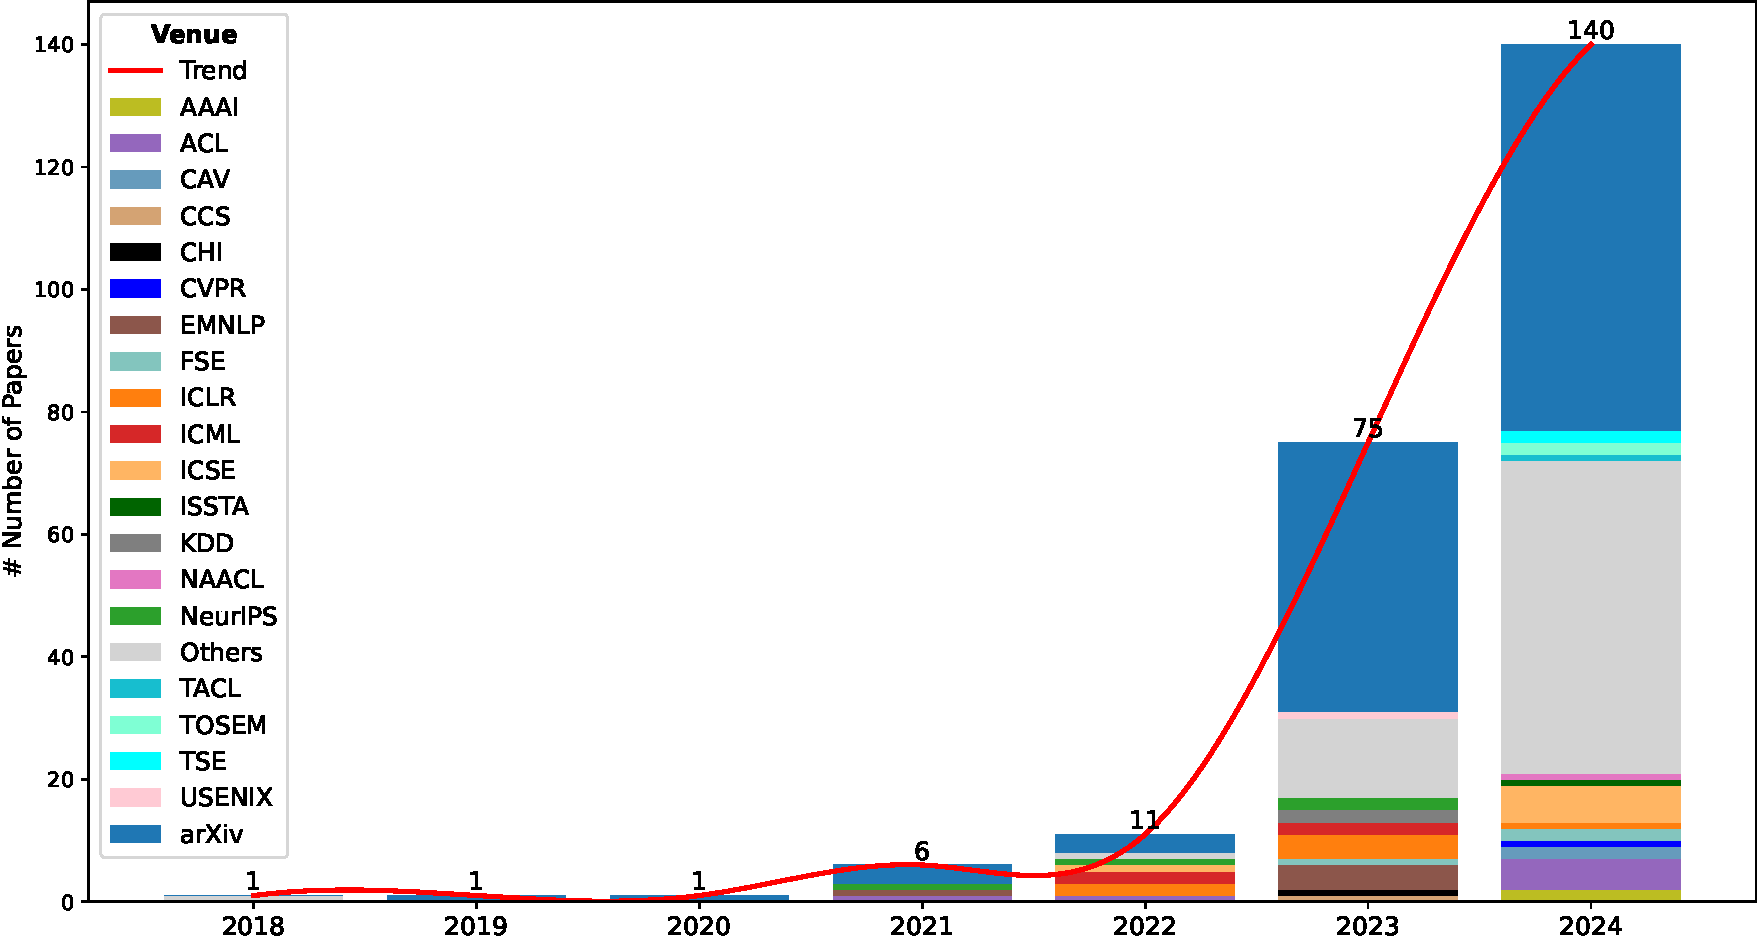
\includegraphics[width=0.95\linewidth]{images/paper_num_bar.pdf}}
%   \subfigure[Distribution of papers over years.]{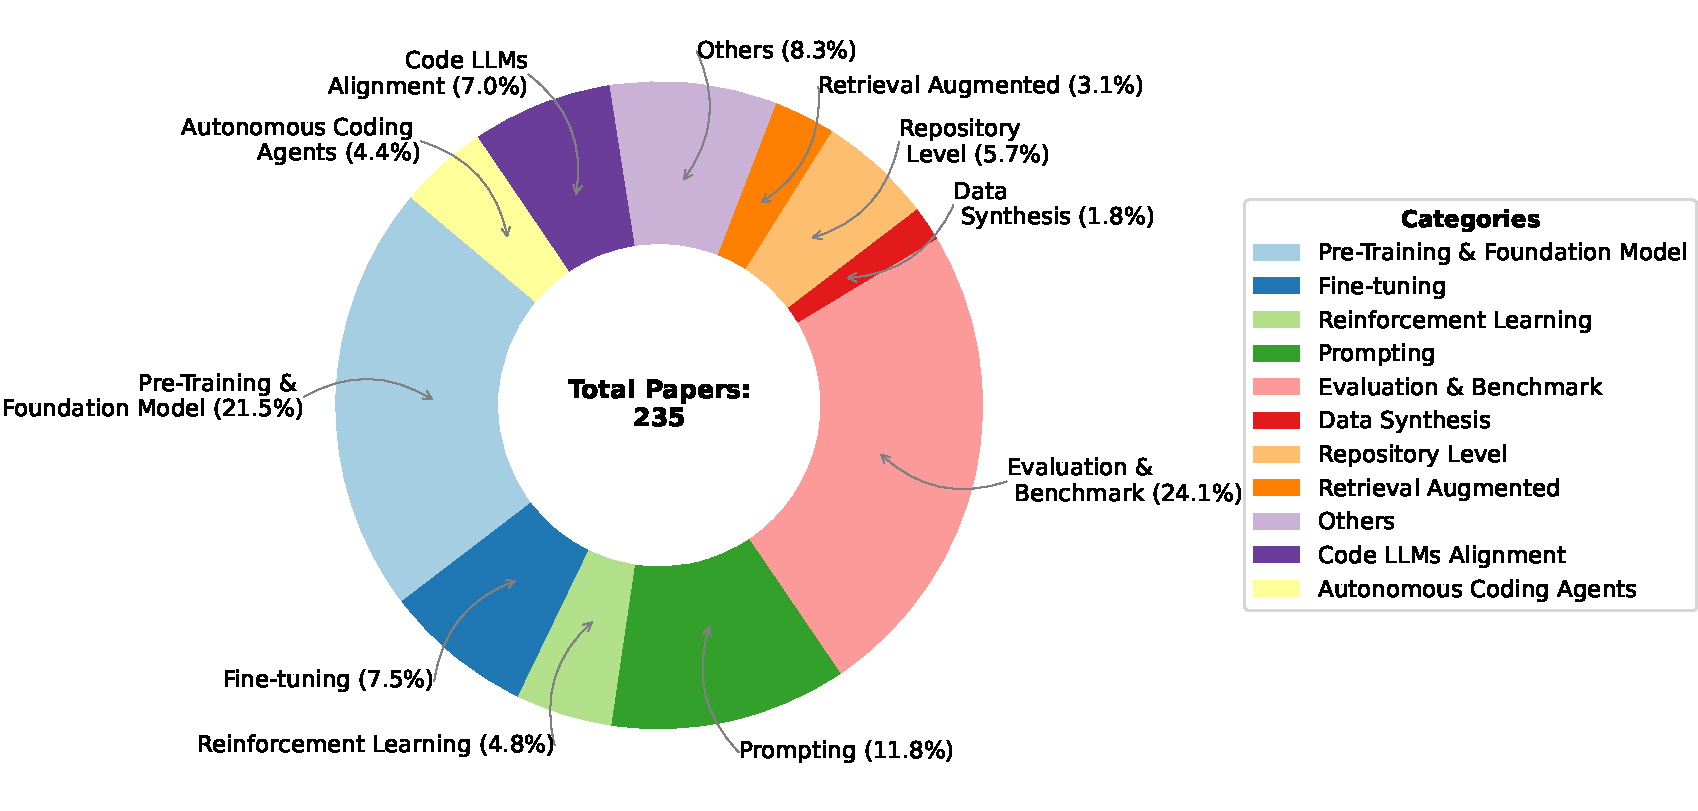
\includegraphics[width=0.95\linewidth]{images/topic_dist_pie.pdf}}
%   \caption{Overview of the selected 235 papers' distribution.}
%   \label{fig:venues_num_topic_dist}
% \end{figure}
\begin{figure}[t]
\centering
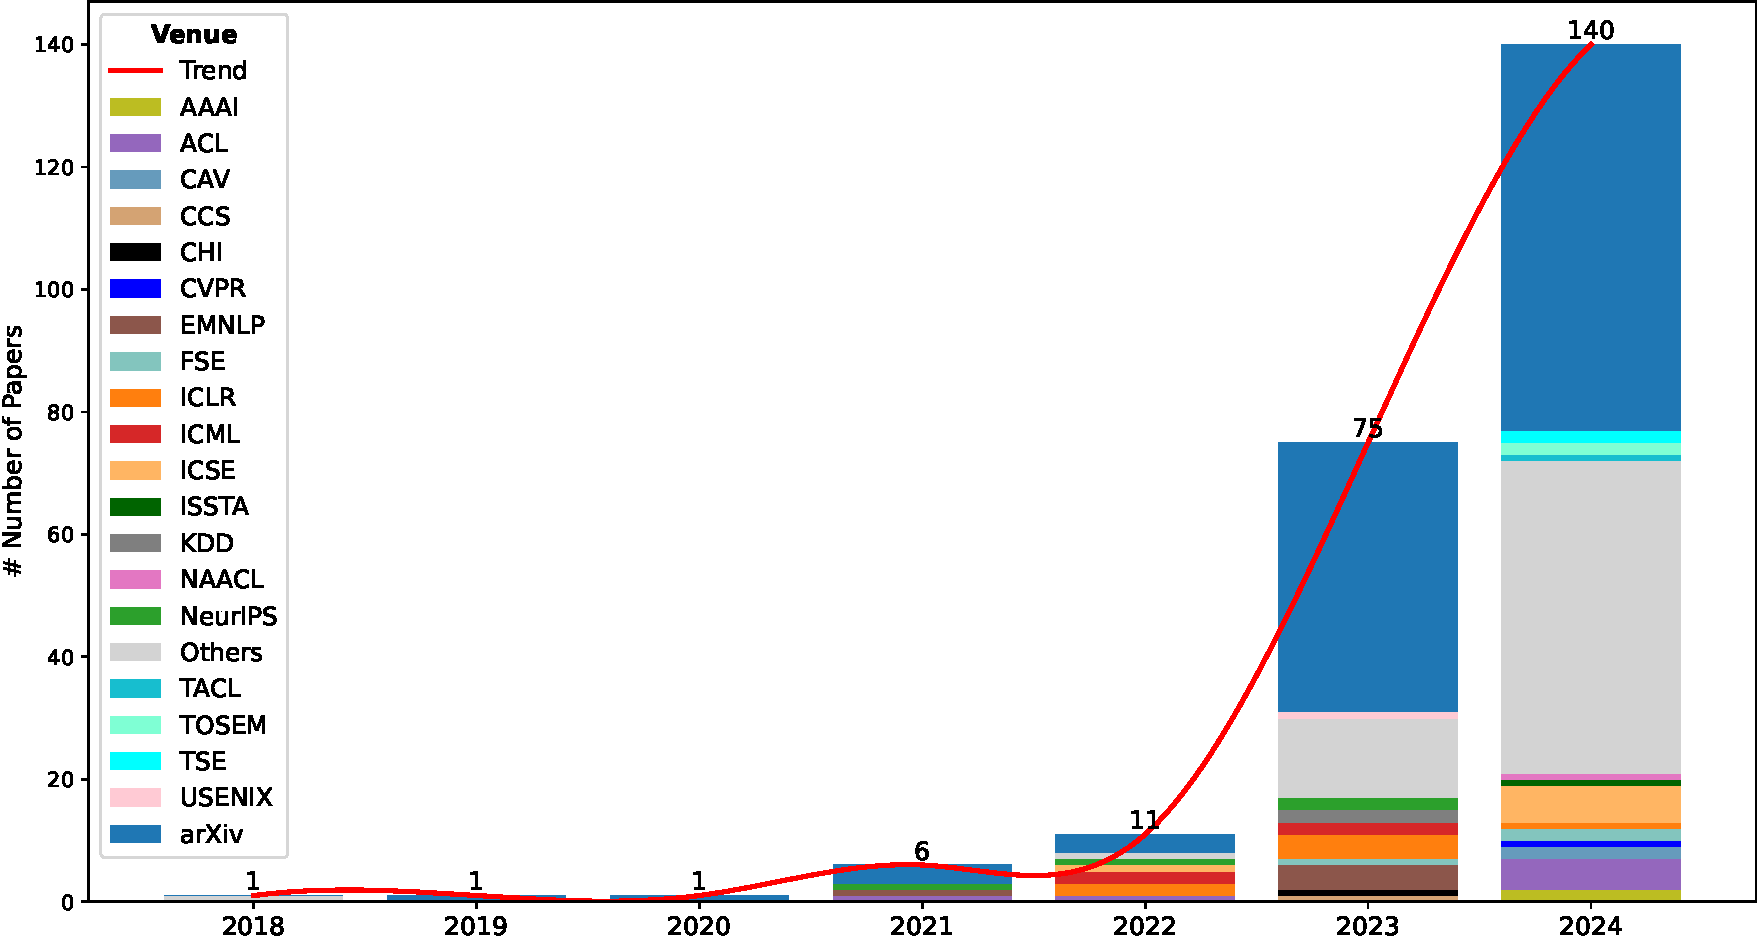
\includegraphics[width=\linewidth]{images/paper_num_bar.pdf}
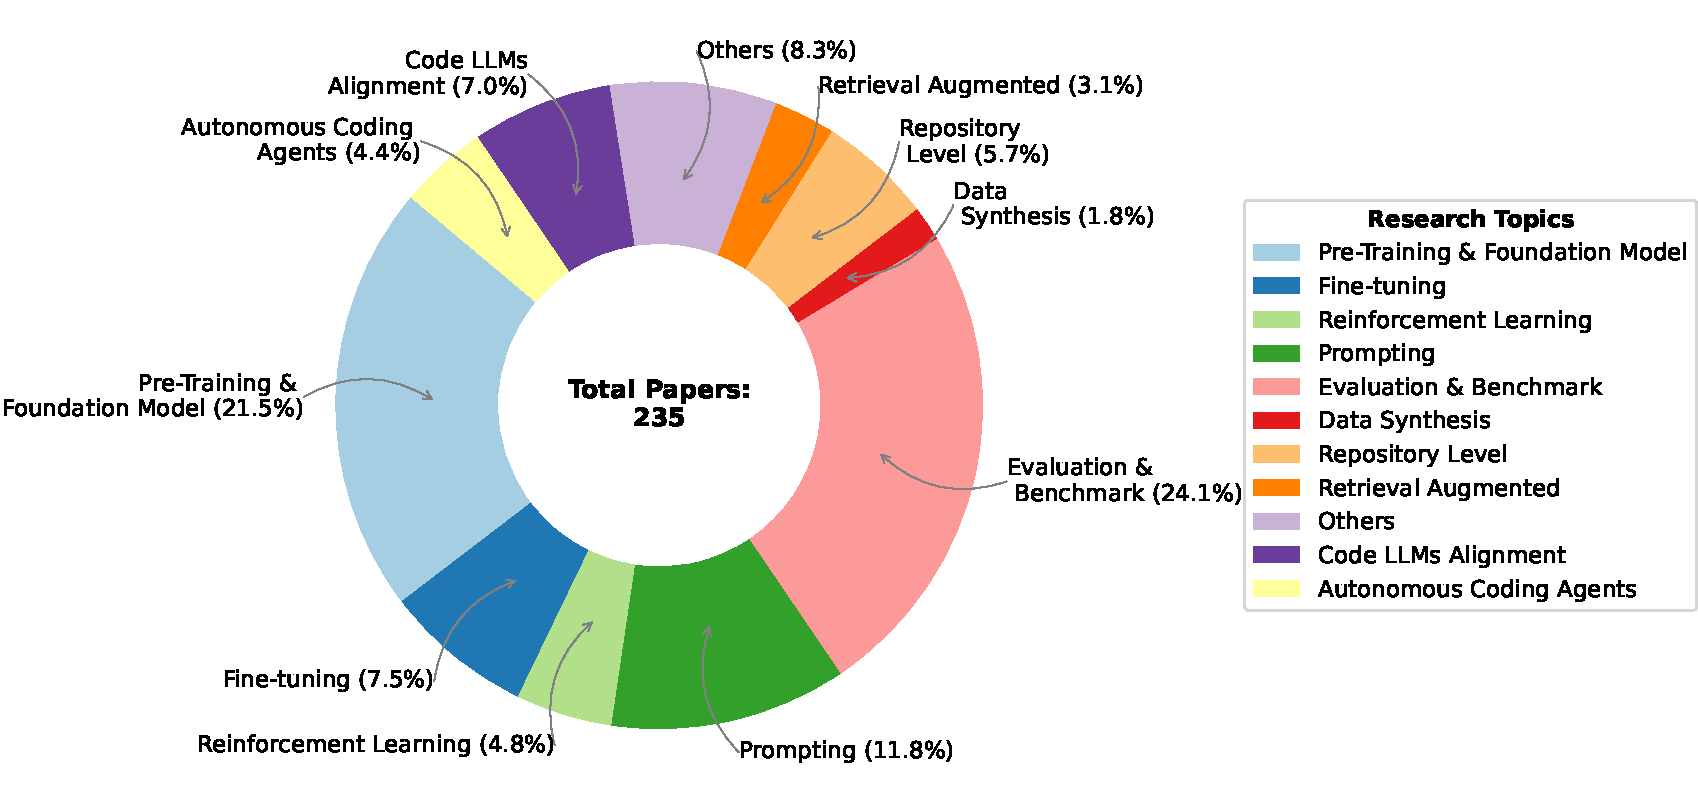
\includegraphics[width=\linewidth]{images/topic_dist_pie_v2.pdf}
\caption{\done{Data qualitative analysis. \textbf{Top}: Annual distribution of selected papers across various publication venues. \textbf{Bottom}: Distribution analysis of research topics covered in the included papers.}}
\label{fig:venues_num_topic_dist}
\end{figure}


\subsection{Data Collection and Analysis}
% As shown in Figure \ref{fig:review_process}, our study collection process started with manual search within the conference proceedings and journal articles from top-tier LLMs and SE venues, resulting in a initial \textcolor{red}{42} papers, to extract search strings from them. 
% Subsequently, we conduct automatic search on four academic databases, employing keywords searching, retrieving a total of \textcolor{red}{14,623} papers. 
% Then after automated filtering, employing inclusion and exclusion criteria, quality assessment, and snowballing, we finally collected a total of \textcolor{red}{192} papers involving LLMs for code generation.
The data collection process for our study, illustrated in Figure \ref{fig:review_process}, began with a manual search through conference proceedings and journal articles from leading venues in LLMs and SE. This initial step yielded 42 papers, from which we extracted relevant search strings. Following this, we performed an automated search across four academic databases using keyword-based queries, resulting in the retrieval of 664 papers. After performing automatic filtering (351 papers), applying inclusion and exclusion criteria (247 papers), conducting quality assessments (235 papers), and utilizing snowballing search (235 papers), we finalize a collection of 235 papers focusing on LLMs for code generation.

% To provide some insights from included papers, we presents an overview of the distribution of the included papers across LLMs and SE publication venues, as depicted in Figure \ref{fig:venues_num_topic_dist}(a).
% We observe that 47\% papers are published in software engineering venues, among which 19 papers are from ICSE, 5 papers are from FSE, 5 papers are from ASE, and 3 papers are from ISSTA. 
% 2\% papers are published in artificial intelligence venues such as EMNLP and ICLR, and 5\% papers are published in program analysis or security venues like PLDI and S\&P. 
% Besides, 46\% of the papers have not yet been published via peer-reviewed venues, i.e., they are disclosed on arXiv. This is understandable because this field is emerging and many works are just completed and in the process of submission. Although these papers did not undergo peer review, we have a quality assessment process that eliminates papers with low quality, which potentially ensures the quality of this survey. 
% Moreover, we demonstrate the trend of our collected papers per year in Figure \ref{fig:venues_num_topic_dist}(b). 
% We can see that as the years go by, the number of papers in this field is growing almost exponentially. 
% In 2020 and 2021, there were only 1 and 2 papers, respectively. 
% In 2022, there were 19 papers, and in 2023, there have been 82 papers. It is conceivable that there will be even more papers in the future, which indicates the popularity and attention that this field is receiving.
% To provide a wide spectrum of cutting-edge progress in LLMs for code generation, we further conducted a distribution analysis of various advanced techniques and topics involved in included papers, as illustrated in Figure \ref{fig:venues_num_topic_dist}(c).
% We can see that LLMs for code generation essentially aligns with the development of LLMs.  
% Specifically, data synthesis, reinforcement learning with feedback, and prompting engineering are the three most popular topics, indicating that these three topics have a more promising to enhance and refine the code generation with LLMs.

% To provide insights from the selected papers, we first present an overview of their distribution of venues across each year in the top of Figure \ref{fig:venues_num_topic_dist}. Our analysis reveals that 14\% were published in LLMs venues and 7\% of the papers were published in SE venues, while notably, 49\% of the papers remain unpublished in peer-reviewed venues, being available on arXiv. 
% This is understandable given the nascent nature of this field, where many works are recent and pending submission. Despite the lack of peer review in arXiv, our quality assessment process ensures the inclusion of only high-quality papers, thereby maintaining the integrity of this survey.
% Furthermore, the annual trend in the number of collected papers demonstrates that the field has experienced nearly exponential growth, with only 1 paper in 2018 to 2020, 6 in 2021, 11 in 2022, 75 in 2023, and 140 in 2024. This trend suggests increasing interest and attention in this research area, with expectations for continued growth in the future.
% Moreover, to capture the breadth of advancements in LLMs for code generation, we conducted a distribution analysis of the research topics covered in the included papers, as shown in the bottom of Figure \ref{fig:venues_num_topic_dist}. 
% We observe that the development of LLMs for code generation closely mirrors broader trends in LLM research. 
% Notably, evaluation \& benchmarks (24.1\%), pre-training \& foundation model (21.5\%), and prompting (11.8\%) are the most three prevalent research topics. 
% These research topics hold significant promise for enhancing and refining LLM-driven code generation.
To provide insights from the selected papers, we begin by presenting an overview of their distribution across publication venues each year, as illustrated at the top of Figure \ref{fig:venues_num_topic_dist}. 
Our analysis indicates that 14\% of the papers are published in LLM-specific venues and 7\% in SE venues. Remarkably, 49\% of the papers remain unpublished in peer-reviewed venues and are available on arXiv. 
This trend is understandable given the emerging nature of this field, with many works being recent and pending formal submission. 
Despite the absence of peer review on arXiv, our quality assessment process ensures that only high-quality papers are included, thereby maintaining the integrity of this survey.
Furthermore, the annual trend in the number of collected papers indicates nearly exponential growth in the field. From a single paper in the period 2018 to 2020, the numbers increased to 6 in 2021, 11 in 2022, 75 in 2023, and 140 in 2024. This trend reflects growing interest and attention in this research area, with expectations for continued expansion in the future.
Additionally, to capture the breadth of advancements in LLMs for code generation, we conducted a distribution analysis of the research topics covered in the included papers, as shown at the bottom of Figure \ref{fig:venues_num_topic_dist}. We observe that the development of LLMs for code generation closely aligns with broader trends in general-purpose LLM research. Notably, the most prevalent research topics are Pre-training and Foundation Models (21.5\%), Prompting (11.8\%), and Evaluation and Benchmarks (24.1\%). These areas hold significant promise for enhancing, refining, and evaluating LLM-driven code generation.


% Researchers gradually adapts the general techniques and topics of LLMs into the code generation task.